\documentclass[]{article}
\usepackage{lmodern}
\usepackage{amssymb,amsmath}
\usepackage{ifxetex,ifluatex}
\usepackage{fixltx2e} % provides \textsubscript
\ifnum 0\ifxetex 1\fi\ifluatex 1\fi=0 % if pdftex
  \usepackage[T1]{fontenc}
  \usepackage[utf8]{inputenc}
\else % if luatex or xelatex
  \ifxetex
    \usepackage{mathspec}
  \else
    \usepackage{fontspec}
  \fi
  \defaultfontfeatures{Ligatures=TeX,Scale=MatchLowercase}
\fi
% use upquote if available, for straight quotes in verbatim environments
\IfFileExists{upquote.sty}{\usepackage{upquote}}{}
% use microtype if available
\IfFileExists{microtype.sty}{%
\usepackage{microtype}
\UseMicrotypeSet[protrusion]{basicmath} % disable protrusion for tt fonts
}{}
\usepackage[margin=1in]{geometry}
\usepackage{hyperref}
\hypersetup{unicode=true,
            pdftitle={mini-project-2},
            pdfauthor={Akash Mahajan (akashmjn@stanford.edu), Raunaq Rewari (raunaq@stanford.edu)},
            pdfborder={0 0 0},
            breaklinks=true}
\urlstyle{same}  % don't use monospace font for urls
\usepackage{color}
\usepackage{fancyvrb}
\newcommand{\VerbBar}{|}
\newcommand{\VERB}{\Verb[commandchars=\\\{\}]}
\DefineVerbatimEnvironment{Highlighting}{Verbatim}{commandchars=\\\{\}}
% Add ',fontsize=\small' for more characters per line
\usepackage{framed}
\definecolor{shadecolor}{RGB}{248,248,248}
\newenvironment{Shaded}{\begin{snugshade}}{\end{snugshade}}
\newcommand{\KeywordTok}[1]{\textcolor[rgb]{0.13,0.29,0.53}{\textbf{{#1}}}}
\newcommand{\DataTypeTok}[1]{\textcolor[rgb]{0.13,0.29,0.53}{{#1}}}
\newcommand{\DecValTok}[1]{\textcolor[rgb]{0.00,0.00,0.81}{{#1}}}
\newcommand{\BaseNTok}[1]{\textcolor[rgb]{0.00,0.00,0.81}{{#1}}}
\newcommand{\FloatTok}[1]{\textcolor[rgb]{0.00,0.00,0.81}{{#1}}}
\newcommand{\ConstantTok}[1]{\textcolor[rgb]{0.00,0.00,0.00}{{#1}}}
\newcommand{\CharTok}[1]{\textcolor[rgb]{0.31,0.60,0.02}{{#1}}}
\newcommand{\SpecialCharTok}[1]{\textcolor[rgb]{0.00,0.00,0.00}{{#1}}}
\newcommand{\StringTok}[1]{\textcolor[rgb]{0.31,0.60,0.02}{{#1}}}
\newcommand{\VerbatimStringTok}[1]{\textcolor[rgb]{0.31,0.60,0.02}{{#1}}}
\newcommand{\SpecialStringTok}[1]{\textcolor[rgb]{0.31,0.60,0.02}{{#1}}}
\newcommand{\ImportTok}[1]{{#1}}
\newcommand{\CommentTok}[1]{\textcolor[rgb]{0.56,0.35,0.01}{\textit{{#1}}}}
\newcommand{\DocumentationTok}[1]{\textcolor[rgb]{0.56,0.35,0.01}{\textbf{\textit{{#1}}}}}
\newcommand{\AnnotationTok}[1]{\textcolor[rgb]{0.56,0.35,0.01}{\textbf{\textit{{#1}}}}}
\newcommand{\CommentVarTok}[1]{\textcolor[rgb]{0.56,0.35,0.01}{\textbf{\textit{{#1}}}}}
\newcommand{\OtherTok}[1]{\textcolor[rgb]{0.56,0.35,0.01}{{#1}}}
\newcommand{\FunctionTok}[1]{\textcolor[rgb]{0.00,0.00,0.00}{{#1}}}
\newcommand{\VariableTok}[1]{\textcolor[rgb]{0.00,0.00,0.00}{{#1}}}
\newcommand{\ControlFlowTok}[1]{\textcolor[rgb]{0.13,0.29,0.53}{\textbf{{#1}}}}
\newcommand{\OperatorTok}[1]{\textcolor[rgb]{0.81,0.36,0.00}{\textbf{{#1}}}}
\newcommand{\BuiltInTok}[1]{{#1}}
\newcommand{\ExtensionTok}[1]{{#1}}
\newcommand{\PreprocessorTok}[1]{\textcolor[rgb]{0.56,0.35,0.01}{\textit{{#1}}}}
\newcommand{\AttributeTok}[1]{\textcolor[rgb]{0.77,0.63,0.00}{{#1}}}
\newcommand{\RegionMarkerTok}[1]{{#1}}
\newcommand{\InformationTok}[1]{\textcolor[rgb]{0.56,0.35,0.01}{\textbf{\textit{{#1}}}}}
\newcommand{\WarningTok}[1]{\textcolor[rgb]{0.56,0.35,0.01}{\textbf{\textit{{#1}}}}}
\newcommand{\AlertTok}[1]{\textcolor[rgb]{0.94,0.16,0.16}{{#1}}}
\newcommand{\ErrorTok}[1]{\textcolor[rgb]{0.64,0.00,0.00}{\textbf{{#1}}}}
\newcommand{\NormalTok}[1]{{#1}}
\usepackage{graphicx,grffile}
\makeatletter
\def\maxwidth{\ifdim\Gin@nat@width>\linewidth\linewidth\else\Gin@nat@width\fi}
\def\maxheight{\ifdim\Gin@nat@height>\textheight\textheight\else\Gin@nat@height\fi}
\makeatother
% Scale images if necessary, so that they will not overflow the page
% margins by default, and it is still possible to overwrite the defaults
% using explicit options in \includegraphics[width, height, ...]{}
\setkeys{Gin}{width=\maxwidth,height=\maxheight,keepaspectratio}
\IfFileExists{parskip.sty}{%
\usepackage{parskip}
}{% else
\setlength{\parindent}{0pt}
\setlength{\parskip}{6pt plus 2pt minus 1pt}
}
\setlength{\emergencystretch}{3em}  % prevent overfull lines
\providecommand{\tightlist}{%
  \setlength{\itemsep}{0pt}\setlength{\parskip}{0pt}}
\setcounter{secnumdepth}{0}
% Redefines (sub)paragraphs to behave more like sections
\ifx\paragraph\undefined\else
\let\oldparagraph\paragraph
\renewcommand{\paragraph}[1]{\oldparagraph{#1}\mbox{}}
\fi
\ifx\subparagraph\undefined\else
\let\oldsubparagraph\subparagraph
\renewcommand{\subparagraph}[1]{\oldsubparagraph{#1}\mbox{}}
\fi

%%% Use protect on footnotes to avoid problems with footnotes in titles
\let\rmarkdownfootnote\footnote%
\def\footnote{\protect\rmarkdownfootnote}

%%% Change title format to be more compact
\usepackage{titling}

% Create subtitle command for use in maketitle
\newcommand{\subtitle}[1]{
  \posttitle{
    \begin{center}\large#1\end{center}
    }
}

\setlength{\droptitle}{-2em}
  \title{mini-project-2}
  \pretitle{\vspace{\droptitle}\centering\huge}
  \posttitle{\par}
  \author{Akash Mahajan
(\href{mailto:akashmjn@stanford.edu}{\nolinkurl{akashmjn@stanford.edu}}),
Raunaq Rewari
(\href{mailto:raunaq@stanford.edu}{\nolinkurl{raunaq@stanford.edu}})}
  \preauthor{\centering\large\emph}
  \postauthor{\par}
  \date{}
  \predate{}\postdate{}


\begin{document}
\maketitle

\subsection{Recap - Spotify's Worldwide Daily Song
Ranking}\label{recap---spotifys-worldwide-daily-song-ranking}

To recall, we are working with a dataset containing streams for the
daily top 200 songs, over a span of 226 days in 2017 (Starting Jan 1st),
containing 53 regions totally, as well as global charts. Our data in its
raw form looks as below, consisting of Date, Region, TrackName Streams,
Artist, Position (on top 200), URL. This corresponds to 916600 rows
totally, with the URL serving as a unqiue ID for a track.

To simplify our problem, we focus our attention on only the top 20
regions, effectively those having mean daily streams of
\(\geq\sim 13,000\).

\begin{verbatim}
## Warning in gmean(Streams): Group 6 summed to more than type 'integer'
## can hold so the result has been coerced to 'numeric' automatically, for
## convenience.
\end{verbatim}

\begin{verbatim}
##    Region Position         TrackName         Artist Streams
## 1: global        1          Mi Gente       J Balvin 4553972
## 2: global        2 Despacito - Remix     Luis Fonsi 3510238
## 3: global        3     Unforgettable French Montana 3369525
## 4: global        4     Wild Thoughts      DJ Khaled 3311014
## 5: global        5             Feels  Calvin Harris 3178439
##                                                      URL       Date
## 1: https://open.spotify.com/track/2rb5MvYT7ZIxbKW5hfcHx8 2017-08-17
## 2: https://open.spotify.com/track/5CtI0qwDJkDQGwXD1H1cLb 2017-08-17
## 3: https://open.spotify.com/track/3B54sVLJ402zGa6Xm4YGNe 2017-08-17
## 4: https://open.spotify.com/track/1OAh8uOEOvTDqkKFsKksCi 2017-08-17
## 5: https://open.spotify.com/track/5bcTCxgc7xVfSaMV3RuVke 2017-08-17
##    MeanStreams
## 1:     1037953
## 2:     1037953
## 3:     1037953
## 4:     1037953
## 5:     1037953
\end{verbatim}

\subsection{Problem Formulation}\label{problem-formulation}

\subsubsection{Transformation /
Discretization}\label{transformation-discretization}

While our dataset looks deceptively simple in form, it is also fairly
unstructured, consisting of about \textasciitilde{}19000 partial time
series values for each unique (Track,Region) in the recorded period.
These are partial, since a song may enter/leave the top 200 for only a
small period of time. Thus building on some of the open questions from
our previous report, we've done some further exploration before posing
our problem. Our primary motivation is - can we spot any potential
trends in song streams that indicate a rise in popularity, to say Top
50?

We first make sure that we are working with songs that only have fairly
complete durations of streams present. Looking at how the tracks are
distributed, we confirm our expectation that a good number are present
for a very small number of days (\textless{}10-15). We arbitrarily set a
threshold at d=28 days (i.e.~4 weeks), bringing down the total number of
tracks/time series to \textasciitilde{}8300.

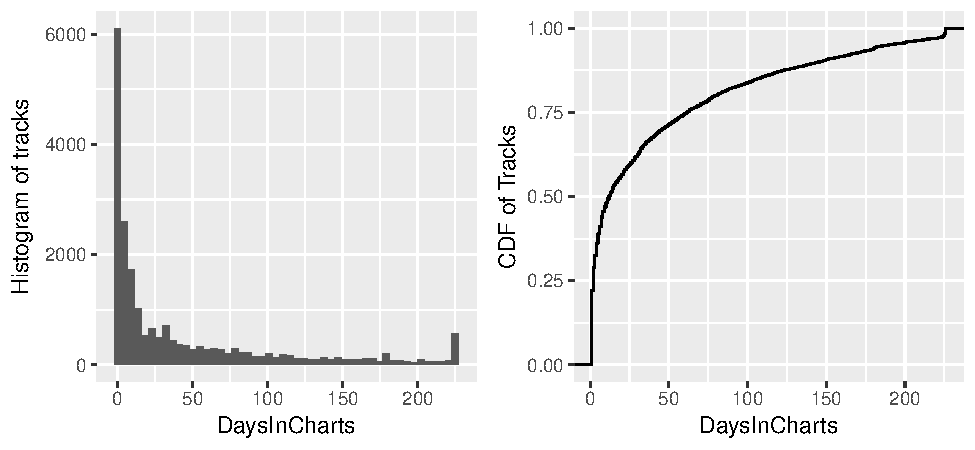
\includegraphics{report-2_files/figure-latex/tsdurations-1.pdf}

Finally, we split these songs into discrete categories, based on an
arbitrary popularity category such as Top 50, 100, etc. (Note that top
200 constitutes our entire dataset). These tracks are then randomly
sampled, to constitute our training/test datasets.

For illustration purposes, trends for songs that have made it to the top
50 at some point over our period of interest, are plotted below.

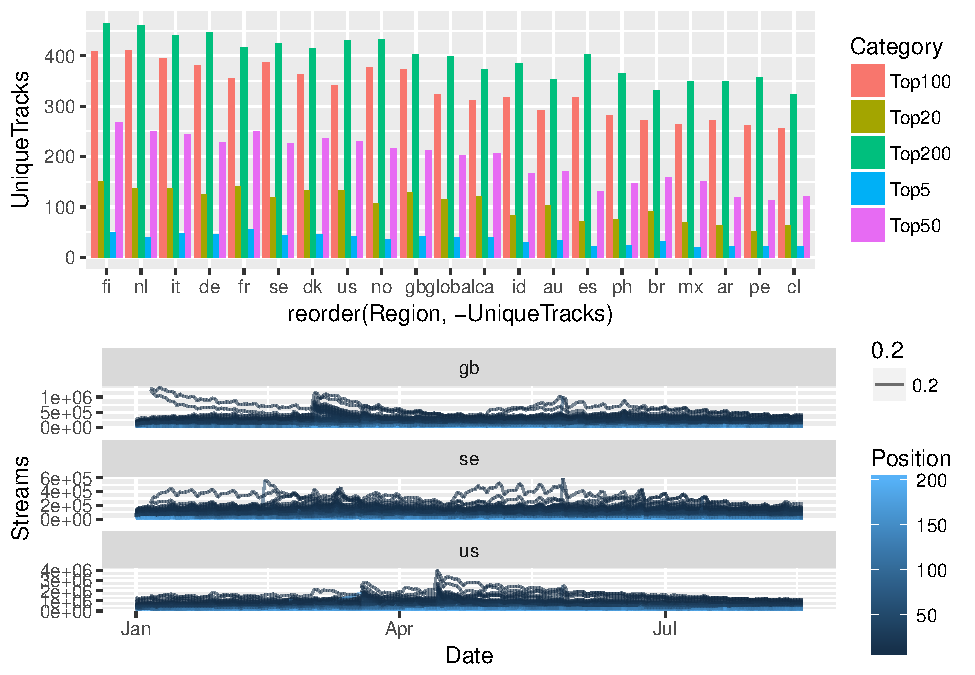
\includegraphics{report-2_files/figure-latex/regionvariation-1.pdf}

\subsubsection{Formulating prediction
tasks}\label{formulating-prediction-tasks}

\begin{itemize}
\tightlist
\item
  Classification: Given external data about track from the Spotify API,
  such as genre, artist, and the region from our dataset, can we predict
  the category labels?
\item
  Regression: For songs in the top 5, can we forecast the number of
  streams, looking ahead a certain period (say 10 days)?
\end{itemize}

The classification task output would be useful to explore at a
high-level what correlates with song popularity.

The regression task output could be useful in helping estimate how long
a song that has made it to the top of the charts actually stays there.

\subsection{Prediction Progress}\label{prediction-progress}

\subsubsection{Regression task}\label{regression-task}

\paragraph{Baseline}\label{baseline}

A baseline for this task would be to just predict the mean of the data.
We use the RMSE as an evaluation metric to compare against. Our RMSE is
143479.02 (this is high since the scale of our data is relatively high
as well).

\begin{verbatim}
## [1] "RMSE for baseline: 143479.02"
\end{verbatim}

\paragraph{Approach}\label{approach}

For an initial simple analysis, we choose just the GB region with about
41 tracks that have made it to the top 5. We randomly set aside (25\%)
\textasciitilde{} 10 tracks that we will not use during our model
building purposes.

We plan to explore the use of time series models for forecasting these
streams. We make use of an ARIMA model that effectively regresses on
values at a previous time instance. An ARMA(p,q,d) model can be
expressed as below (while the I component refers to differencing of the
series, done to eliminate a non-zero mean)

\[
X_t - \alpha_1X_{t-1}, \cdots, -\alpha_pX_{t-p} = \epsilon_t +\theta_1\epsilon_{t-1},\cdots,+\theta_q\epsilon_{t-q} 
\]

To get an idea of model performance, we just evaluate a best fitted
model on a randomly chosen sample of the training songs.

Model selection (between differently parameterized models for p,q,d), is
done using in-sample estimates of the generalization error, namely the
AIC via the R package used.

\begin{verbatim}
## Series: trainTS1 
## ARIMA(2,1,2) with drift 
## 
## Coefficients:
##           ar1     ar2     ma1      ma2     drift
##       -0.4667  0.1850  0.3784  -0.5292  -571.077
## s.e.   0.1560  0.1414  0.1348   0.1289   609.141
## 
## sigma^2 estimated as 192301898:  log likelihood=-2462.97
## AIC=4937.93   AICc=4938.32   BIC=4958.43
## 
## Training set error measures:
##                    ME     RMSE      MAE        MPE     MAPE      MASE
## Training set 138.0933 13681.98 9071.879 -0.3040158 5.905335 0.9987258
##                    ACF1
## Training set 0.01411492
\end{verbatim}

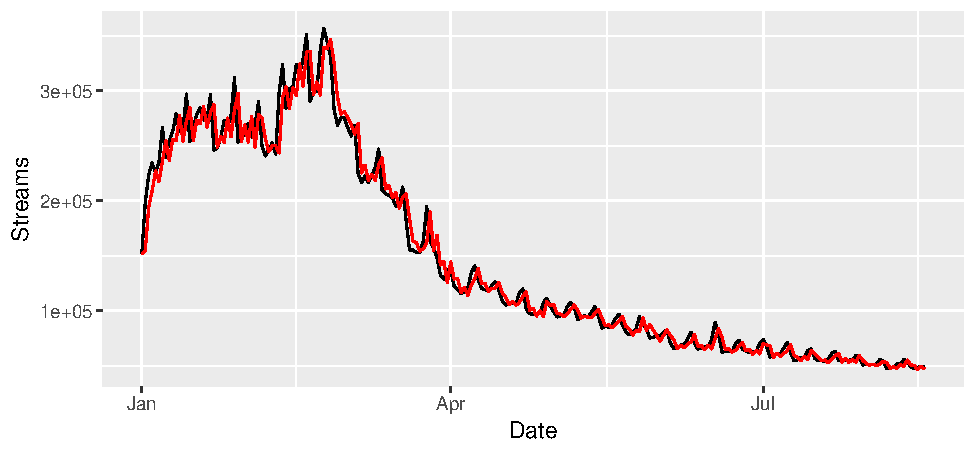
\includegraphics{report-2_files/figure-latex/regress2-1.pdf}
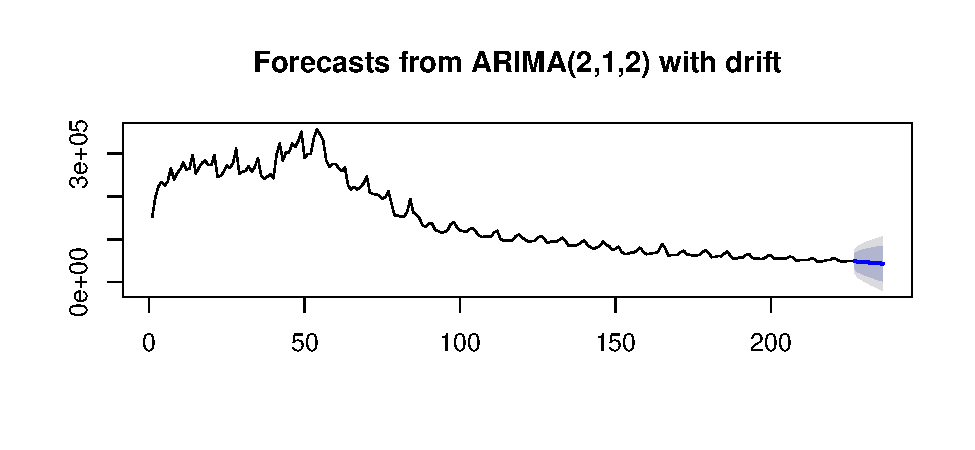
\includegraphics{report-2_files/figure-latex/regress2-2.pdf}

While as expected, the RMSE for our model is lower than the baseline, we
need further work on dealing with a couple of challenges as outlined
below.

\subsubsection{Open Questions}\label{open-questions}

While we have only done a very basic exploration, there's fair amount of
work we need to do to tie this together.

\begin{enumerate}
\def\labelenumi{\arabic{enumi}.}
\item
  How do we valide time series models for many different tracks? Do we
  fit many individual time series models? Do we fit one model per
  region?
\item
  A classification task on our dataset seems a little difficult to pose,
  hence for the classification setting, we looked at trying to predict
  top 20 potential for a song based on the audio features of the song.
\end{enumerate}

To get the audio features, we used Spotify's API that returns the
following features, given the song id:

\begin{verbatim}
•   danceability
•   energy
•   key
•   loudness
•   mode
•   speechiness
•   acousticness
•   instrumentalness
•   liveness
•   valence
•   tempo
\end{verbatim}

For this task, we also modified the dataset to make it amenable to the
classification setting. Any song that had a position within top 20 was
given a label 1 and 0 otherwise.

We have not included the classification results here (even though we
have attached the relevant code) because we weren't confident about the
results. This was mainly because the same song (with the same features)
is represented multiple times in the dataset, across multiple regions.

We are working on making modifications for the same to conclude our
analysis.

\newpage

\subsection{Source Code}\label{source-code}

\begin{Shaded}
\begin{Highlighting}[]
\NormalTok{##### Helper functions used #######}

\CommentTok{# Filter and return top N regions }
\NormalTok{getTopNRegions <-}\StringTok{ }\NormalTok{function(dt,N)\{}
  \CommentTok{# Mean of streams by region}
  \NormalTok{dailyStreamsByRegion =}\StringTok{ }\NormalTok{dt[,.(}\DataTypeTok{MeanStreams=}\KeywordTok{mean}\NormalTok{(Streams)),by=Region]}
  \CommentTok{# filter by region - only top 20 regions}
  \NormalTok{topNRegions =}\StringTok{ }\NormalTok{dailyStreamsByRegion[}\KeywordTok{order}\NormalTok{(-MeanStreams)][}\DecValTok{1}\NormalTok{:(N}\DecValTok{+1}\NormalTok{)]}
  \NormalTok{dtFiltered =}\StringTok{ }\KeywordTok{merge}\NormalTok{(dt,topNRegions,}\DataTypeTok{by =} \StringTok{"Region"}\NormalTok{)}
  \KeywordTok{return}\NormalTok{(dtFiltered)}
\NormalTok{\}}

\CommentTok{# Filter only tracks that have been in the top N }
\CommentTok{# charts by region. N=200 will just return the entire dataset}
\CommentTok{# Returns: list( dtFiltered, topNTracksStats )}
\NormalTok{getTopNTracks <-}\StringTok{ }\NormalTok{function(dt,N)\{}
  \CommentTok{# filter tracks getting <= N ranking at some point}
  \CommentTok{# groupby TrackName, Region gives a count of dates }
  \NormalTok{topNTracksByRegion =}\StringTok{ }\NormalTok{dt[Position<=N][,}
                               \NormalTok{.(}\DataTypeTok{DaysInTopN=}\NormalTok{.N),}
                               \NormalTok{by=.(TSID,Region)]}
  \CommentTok{# join and filter only tracks in this topN list}
  \NormalTok{dtFiltered =}\StringTok{ }\KeywordTok{merge}\NormalTok{(dt,topNTracksByRegion,}\DataTypeTok{by=}\KeywordTok{c}\NormalTok{(}\StringTok{"TSID"}\NormalTok{,}\StringTok{"Region"}\NormalTok{))}
  \KeywordTok{return}\NormalTok{(}\KeywordTok{list}\NormalTok{(dtFiltered,topNTracksByRegion))}
\NormalTok{\}}

\CommentTok{# filter valid time series }
\CommentTok{# Returns: list( dtFiltered, dtTSDurations )}
\NormalTok{filterValidTS <-}\StringTok{ }\NormalTok{function(dt,minDaysThresh)\{}
  \CommentTok{# pulling out time series with minimum days present }
  \NormalTok{dtTSDurations =}\StringTok{ }\NormalTok{dt[,.(}\DataTypeTok{DaysInCharts=}\NormalTok{.N),by=.(URL,Region)][DaysInCharts>=minDaysThresh]}
  \CommentTok{# giving each time series and ID}
  \NormalTok{dtTSDurations[,TSID:}\ErrorTok{=}\NormalTok{.I]}
  \CommentTok{# joining and filtering back on original dataset}
  \NormalTok{dtFiltered =}\StringTok{ }\KeywordTok{merge}\NormalTok{(dt,dtTSDurations[,.(TSID,Region,URL)],}\DataTypeTok{by =} \KeywordTok{c}\NormalTok{(}\StringTok{"URL"}\NormalTok{,}\StringTok{"Region"}\NormalTok{))}
  \KeywordTok{return}\NormalTok{(}\KeywordTok{list}\NormalTok{(dtFiltered,dtTSDurations))}
\NormalTok{\}}

\NormalTok{######  Notebook code ########}

\NormalTok{## Data preparation }

\CommentTok{# loading in script files}
\KeywordTok{source}\NormalTok{(}\StringTok{"src_akash.R"}\NormalTok{)}

\NormalTok{dt =}\StringTok{ }\KeywordTok{fread}\NormalTok{(}\StringTok{"data.csv"}\NormalTok{)  }\CommentTok{# faster than read.csv }
\KeywordTok{setnames}\NormalTok{(dt,}\StringTok{"Track Name"}\NormalTok{,}\StringTok{"TrackName"}\NormalTok{)}
\NormalTok{dt[,Date:}\ErrorTok{=}\KeywordTok{as.Date}\NormalTok{(Date)]}
\NormalTok{data =}\StringTok{ }\KeywordTok{data.frame}\NormalTok{(dt)}
\NormalTok{data$Date =}\StringTok{ }\KeywordTok{as.Date}\NormalTok{(data$Date)}

\CommentTok{# Filter to just top 20 regions}
\NormalTok{dt =}\StringTok{ }\KeywordTok{getTopNRegions}\NormalTok{(dt,}\DecValTok{20}\NormalTok{)}

\NormalTok{## Filtering time series by minimum durations}

\NormalTok{dtTSDurations =}\StringTok{ }\NormalTok{dt[,.(}\DataTypeTok{DaysInCharts=}\NormalTok{.N),by=.(URL,Region)]}

\NormalTok{p1 <-}\StringTok{ }\KeywordTok{ggplot}\NormalTok{(dtTSDurations)+}\KeywordTok{geom_histogram}\NormalTok{(}\KeywordTok{aes}\NormalTok{(}\DataTypeTok{x=}\NormalTok{DaysInCharts),}\DataTypeTok{bins=}\DecValTok{50}\NormalTok{)+}\KeywordTok{ylab}\NormalTok{(}\StringTok{"Histogram of tracks"}\NormalTok{)}
\NormalTok{p2 <-}\StringTok{ }\KeywordTok{ggplot}\NormalTok{(dtTSDurations)+}\KeywordTok{stat_ecdf}\NormalTok{(}\KeywordTok{aes}\NormalTok{(}\DataTypeTok{x=}\NormalTok{DaysInCharts))+}\KeywordTok{ylab}\NormalTok{(}\StringTok{"CDF of Tracks"}\NormalTok{)}

\KeywordTok{grid.arrange}\NormalTok{(p1,p2,}\DataTypeTok{nrow=}\DecValTok{1}\NormalTok{)}

\CommentTok{# Filtering down data to only time series of a minium duration}
\CommentTok{# Giving a unique ID to a (Track,Region) pair. (this corresponds to one time series)}
\NormalTok{tsFilterStat =}\StringTok{ }\KeywordTok{filterValidTS}\NormalTok{(dt,}\DecValTok{28}\NormalTok{)}
\NormalTok{dtFilteredTS =}\StringTok{ }\NormalTok{tsFilterStat[[}\DecValTok{1}\NormalTok{]]}
\NormalTok{dtTSDurations =}\StringTok{ }\NormalTok{tsFilterStat[[}\DecValTok{2}\NormalTok{]]}

\NormalTok{## Track Categories}

\CommentTok{# filter tracks by chart positions (top 200 tracks, top 100 tracks, etc.)}
\NormalTok{topUniqueTracks =}\StringTok{ }\KeywordTok{data.table}\NormalTok{()}
\NormalTok{for(N in }\KeywordTok{c}\NormalTok{(}\DecValTok{200}\NormalTok{,}\DecValTok{100}\NormalTok{,}\DecValTok{50}\NormalTok{,}\DecValTok{20}\NormalTok{,}\DecValTok{5}\NormalTok{))\{}
  \NormalTok{stat =}\StringTok{ }\KeywordTok{getTopNTracks}\NormalTok{(dtFilteredTS,N)}
  \NormalTok{topNTracksByRegion =}\StringTok{ }\NormalTok{stat[[}\DecValTok{2}\NormalTok{]]}
  \NormalTok{topUniqueTracks =}\StringTok{ }\KeywordTok{rbind}\NormalTok{(topUniqueTracks,}
                          \NormalTok{topNTracksByRegion[,}
                                      \NormalTok{.(}\DataTypeTok{UniqueTracks=}\NormalTok{.N,}\DataTypeTok{Category=}\KeywordTok{paste0}\NormalTok{(}\StringTok{"Top"}\NormalTok{,N)),}
                                      \DataTypeTok{by=}\NormalTok{Region])}
\NormalTok{\}}

\NormalTok{### Regression }

\NormalTok{## Making a dataset of only top 5 songs }
\NormalTok{nTop =}\StringTok{ }\DecValTok{5}
\NormalTok{topStat =}\StringTok{ }\KeywordTok{getTopNTracks}\NormalTok{(dtFilteredTS,}\DecValTok{5}\NormalTok{)}
\NormalTok{dtTop =}\StringTok{ }\NormalTok{topStat[[}\DecValTok{1}\NormalTok{]]}

\NormalTok{dtTopGB =}\StringTok{ }\NormalTok{dtTop[Region==}\StringTok{'gb'}\NormalTok{]}
\NormalTok{gbTopTSIDs =}\StringTok{ }\KeywordTok{unique}\NormalTok{(dtTopGB$TSID)}

\KeywordTok{set.seed}\NormalTok{(}\DecValTok{3}\NormalTok{)}
\NormalTok{trainTSIDs =}\StringTok{ }\KeywordTok{sample}\NormalTok{(gbTopTSIDs,}\DecValTok{31}\NormalTok{)}

\NormalTok{dtTS =}\StringTok{ }\NormalTok{dtTopGB[TSID==trainTSIDs[}\DecValTok{1}\NormalTok{],.(Streams,Date)]}
\NormalTok{trainTS1 =}\StringTok{ }\KeywordTok{xts}\NormalTok{(dtTS[,Streams],}\DataTypeTok{order.by =} \NormalTok{dtTS[,Date])}

\CommentTok{# Printing RMSE}
\NormalTok{RMSEBaseline =}\StringTok{ }\KeywordTok{sqrt}\NormalTok{(dtTopGB[TSID%in%trainTSIDs,(Streams-}\KeywordTok{mean}\NormalTok{(Streams))^}\DecValTok{2}\NormalTok{,}\DataTypeTok{by=}\NormalTok{TSID][,}\KeywordTok{mean}\NormalTok{(V1)])}

\KeywordTok{print}\NormalTok{(}\KeywordTok{paste}\NormalTok{(}\StringTok{"RMSE for baseline:"}\NormalTok{,}\KeywordTok{round}\NormalTok{(RMSEBaseline,}\DecValTok{2}\NormalTok{) ))}

\NormalTok{tsModel =}\StringTok{ }\KeywordTok{auto.arima}\NormalTok{(trainTS1)}

\KeywordTok{summary}\NormalTok{(tsModel)}

\KeywordTok{ggplot}\NormalTok{(dtTS)+}
\StringTok{  }\KeywordTok{geom_line}\NormalTok{(}\KeywordTok{aes}\NormalTok{(}\DataTypeTok{x=}\NormalTok{Date,}\DataTypeTok{y=}\NormalTok{Streams))+}
\StringTok{  }\KeywordTok{geom_line}\NormalTok{(}\KeywordTok{aes}\NormalTok{(}\DataTypeTok{x=}\NormalTok{Date,}\DataTypeTok{y=}\NormalTok{tsModel$fitted),}\DataTypeTok{color=}\StringTok{'red'}\NormalTok{)}

\KeywordTok{plot}\NormalTok{(}\KeywordTok{forecast}\NormalTok{(tsModel))}

\NormalTok{### Classification }

\CommentTok{# Number of unique songs in the top x }

\NormalTok{x =}\StringTok{ }\DecValTok{20}
\NormalTok{unique_top_20 =}\StringTok{ }\NormalTok{dt %>%}\StringTok{ }\KeywordTok{group_by}\NormalTok{(Region) %>%}\StringTok{ }\KeywordTok{filter}\NormalTok{(Position %in%}\StringTok{ }\KeywordTok{c}\NormalTok{(}\DecValTok{1}\NormalTok{:x)) %>%}\StringTok{ }
\StringTok{  }\KeywordTok{summarise}\NormalTok{(}\DataTypeTok{Total_Unique =} \KeywordTok{n_distinct}\NormalTok{(Track.Name))}

\CommentTok{# Doing a trends analysis for the song "Chantaje" }
\NormalTok{time_series =}\StringTok{ }\NormalTok{dt %>%}\StringTok{ }\KeywordTok{group_by}\NormalTok{(Track.Name, Region) %>%}\StringTok{ }\KeywordTok{filter}\NormalTok{(Track.Name ==}\StringTok{ "Chantaje"}\NormalTok{)}
\NormalTok{top_regions =}\StringTok{ }\NormalTok{(time_series %>%}\StringTok{ }\KeywordTok{group_by}\NormalTok{(Region) %>%}\StringTok{ }
\StringTok{                 }\KeywordTok{summarise}\NormalTok{(}\DataTypeTok{total =} \KeywordTok{n}\NormalTok{()) %>%}\StringTok{ }\KeywordTok{filter}\NormalTok{(total ==}\StringTok{ }\KeywordTok{max}\NormalTok{(total)))$Region}

\NormalTok{time_series %>%}\StringTok{ }\KeywordTok{filter}\NormalTok{(Region %in%}\StringTok{ }\NormalTok{top_regions) %>%}\StringTok{ }
\StringTok{  }\KeywordTok{ggplot}\NormalTok{() +}\StringTok{ }\KeywordTok{geom_point}\NormalTok{(}\DataTypeTok{mapping =} \KeywordTok{aes}\NormalTok{(}\DataTypeTok{x =} \NormalTok{Date, }\DataTypeTok{y =} \NormalTok{Position, }\DataTypeTok{color =} \NormalTok{Region))}

\CommentTok{# Make new dataset with song related features}
\NormalTok{song_feats =}\StringTok{ }\KeywordTok{read_csv}\NormalTok{(}\StringTok{"song_feats.csv"}\NormalTok{)}
\NormalTok{merged =}\StringTok{ }\KeywordTok{merge}\NormalTok{(dt, song_feats, }\DataTypeTok{by=}\StringTok{"URL"}\NormalTok{)}
\NormalTok{merged$label =}\StringTok{ }\KeywordTok{cut}\NormalTok{(merged$Position, }\DataTypeTok{breaks=}\KeywordTok{c}\NormalTok{(}\DecValTok{0}\NormalTok{,}\DecValTok{20}\NormalTok{,}\DecValTok{200}\NormalTok{), }\DataTypeTok{labels=}\KeywordTok{c}\NormalTok{(}\DecValTok{1}\NormalTok{,}\DecValTok{0}\NormalTok{))}

\CommentTok{# Run logistic regression}
\NormalTok{classification =}\StringTok{ }\KeywordTok{glm}\NormalTok{(label ~}\StringTok{ }\NormalTok{energy +}\StringTok{ }\NormalTok{liveness +}\StringTok{ }\NormalTok{tempo +}\StringTok{ }\NormalTok{speechiness +}\StringTok{ }\NormalTok{acousticness +}\StringTok{ }\NormalTok{instrumentalness +}\StringTok{ }\NormalTok{danceability +}\StringTok{ }\NormalTok{loudness, }\DataTypeTok{data =} \NormalTok{merged, }\DataTypeTok{family =} \NormalTok{binomial)}
\end{Highlighting}
\end{Shaded}


\end{document}
